\documentclass[authoryear,preprint]{elsarticle}

\journal{Ann. Nucl. Energy}

\usepackage[breaklinks=true]{hyperref}
\usepackage{listings}
\usepackage{color}

\definecolor{gray}{rgb}{0.4,0.4,0.4}
\definecolor{darkblue}{rgb}{0.0,0.0,0.6}
\definecolor{cyan}{rgb}{0.0,0.6,0.6}

\hypersetup{colorlinks=true,
  pdftitle={The OpenMC Monte Carlo particle transport code},
  pdfauthor={Paul K. Romano and Benoit Forget}}
\def \figureautorefname {Fig.}

\lstset{
  basicstyle=\footnotesize\ttfamily,
  columns=fullflexible,
  showstringspaces=false,
  commentstyle=\color{gray}\upshape,
  frame=single
}

\lstdefinelanguage{XML}
{
  morestring=[b]",
  morestring=[s]{>}{<},
  morecomment=[s]{<?}{?>},
  morecomment=[s]{<!--}{-->},
  stringstyle=\color{black},
  identifierstyle=\color{darkblue},
  keywordstyle=\color{cyan},
  morekeywords={}
}

\begin{document}

\begin{frontmatter}

\title{The OpenMC Monte Carlo particle transport code\tnoteref{t1}}
\author[mit]{Paul K. Romano\corref{cor1}}
\ead{paul.k.romano@gmail.com}
\cortext[cor1]{Corresponding author. Tel.: +1 617 452 3631.}

\author[mit]{Benoit Forget}
\ead{bforget@mit.edu}

\address[mit]{Massachusetts Institute of Technology, Department of Nuclear
  Science and Engineering, 77 Massachusetts Avenue, Building 24-607, Cambridge,
  MA 02139, United States}

\begin{abstract}
A new Monte Carlo code called OpenMC is currently under development at the
Massachusetts Institute of Technology as a tool for simulation on
high-performance computing platforms. Given that many legacy codes do not scale
well on existing and future parallel computer architectures, OpenMC has been
developed from scratch with a focus on high performance scalable algorithms as
well as modern software design practices. The present work describes the methods
used in the OpenMC code and demonstrates the performance and accuracy of the
code on a variety of problems.
\end{abstract}

\begin{keyword}
  Monte Carlo \ neutron transport \ criticality \ high performance computing
  \ open source
\end{keyword}

\end{frontmatter}

\section{Introduction}

The introduction of exascale computing in the next decade will introduce a
variety of challenges both for hardware and software developers. As such,
research and development efforts aimed at enabling high-fidelity, large-scale
simulations that will scale on current and future computer architectures are
currently underway. To support these studies, a new Monte Carlo code has been
under development since early 2011 at the Massachusetts Institute of
Technology. The primary motivation for developing a new Monte Carlo code rather
than using a previously developed code is to have a code that is easily
extensible for research purposes in addition to being high performance, freely
available, and written in a programming language conforming to a contemporary
standard rather than an obsolete language like FORTRAN 77.

\section{Methods}

\subsection{Physics}

The initial work on OpenMC has focused on criticality calculations as applied to
the simulation of nuclear reactors. The solution of the eigenvalue problem
proceeds by the method of successive generations \citep{lieberoth} wherein a
constant number of neutron histories are tracked from birth to death. The data
governing the interaction of neutrons with various nuclei are represented using
the ACE format \citep{ace-format} which is used by MCNP \citep{mcnp} and Serpent
\citep{serpent}. ACE-format data can be generated with the NJOY nuclear data
processing system which converts raw ENDF/B data into linearly-interpolatable data
as required by most Monte Carlo codes. The use of a standard cross section
format allows for a direct comparison of OpenMC with other codes since the same
cross section libraries can be used.

The ACE-format contains continuous-energy cross sections for the following types
of reactions: elastic scattering, fission (or first-chance fission,
second-chance fission, etc.), inelastic scattering, $(n,xn)$, $(n,\gamma)$, and
various other absorption reactions. For those reactions with one or more
neutrons in the exit channel, secondary angle and energy distributions may be
provided. In addition, fissionable nuclides have total, prompt, and/or delayed
$\nu$ as a function of energy and neutron precursor distributions. Many nuclides
also have probability tables to be used for accurate treatment of self-shielding
in the unresolved resonance range. For bound scatterers, separate tables with
$S(\alpha,\beta)$ scattering law data can be used.

One important aspect of a Monte Carlo code is the manner in which macroscopic
cross sections are calculated during a simulation. In general, cross sections
are represented as tabulated functions of energy that are linearly interpolated
between successive values. However, the energy values at which cross sections
are tabulated are different from one nuclide to another. Thus, in order to
determine the total cross section of a material, it may be necessary to do a
binary search on the energy grid of each nuclide within the material. In the
Serpent Monte Carlo code, a unionized energy grid is constructed and used for
all nuclides as described in a recent work by \citet{uniongrid}. The downside of
a unionized energy grid is that the memory requirement may be prohibitively high
for problems with many nuclides.

OpenMC uses an indexing technique to give the same algorithmic benefit of a
unionized grid while requiring much less memory. First, an array of energy
values is constructed that is the union of all points on each nuclide energy
grid. Then, an array of pointers is stored for each nuclide that gives the
corresponding index on the nuclide energy grid for each value on the union
energy grid. This technique does not require that the array of cross sections
for each nuclide be modified in any way; instead, the extra array of pointers
for each nuclide provides a quick means of determining what indices to
interpolate between when calculating a cross section given the index on the
union energy grid.

For neutrons at higher energies, it can be safely assumed that the motion of the
target nucleus is negligible relative to the velocity of the neutron
itself. However, in the thermal and intermediate energy ranges, the target
velocity will alter both the cross sections and the secondary energy and angle
distributions of scattered neutrons. To account for this effect on cross
sections, Doppler broadening is typically performed in the cross section
generation stage. For the angle and energy distributions, OpenMC uses a free gas
approximation \citep{freegas} wherein the velocities of the target nuclei have a
Maxwellian distribution. For thermal neutrons scattering from bound molecules
such as hydrogen or deuterium in water, graphite, and beryllium, the free gas
approximation will not accurately capture the scattering kinematics and
$S(\alpha,\beta)$ scattering law data must be used.

In the unresolved resonance energy range, resonances may be so closely spaced
that it is not possible for experimental measurements to resolve all
resonances. To properly account for self-shielding in this energy range, OpenMC
uses the probability table method \citep{probtables}. For most thermal reactors,
the use of probability tables will not significantly affect problem
results. However, for some fast reactors and other problems with an appreciable
flux spectrum in the unresolved resonance range, not using probability tables
may lead to incorrect results \citep{probtables-testing}.

While extensive variance reduction techniques are not currently available in
OpenMC at the time of this writing, a survival biasing method has been
implemented that can, under certain circumstances, help increase the
figure-of-merit in a Monte Carlo simulation. When survival biasing is used,
absorption never occurs explicitly and instead, a particle's weight is reduced
by the probability that it would have been absorbed at each collision. Weight
cutoffs and Russian rouletting also must be employed to ensure that neutrons of
very low weight are not tracked indefinitely.

\subsection{Geometry}

In order to model arbitrarily complex geometric objects, OpenMC uses a
constructive solid geometry representation. In such a representation, any closed
volume can be represented as the union, intersection, and/or difference of
multiple half-spaces. Each half-space is in turn defined as the positive or
negative side of a plane or quadratic surface. This allows curved surfaces such
as spheres and cylinders to be modeled exactly with no error due to mesh
discretization. Almost all geometries of interest in particle transport can be
modeled with first and second-order surfaces with the exception of some fusion
geometries where a fourth-order torus is required.

As is typical in most Monte Carlo codes, OpenMC provides constructs that allow
the user to model a two or three-dimensional structured mesh consisting of
quadrilaterals or hexagons. These constructs are useful for modeling the core
and assembly layout in a variety of commercial and research reactor designs. As
in MCNP and Serpent, these repeated structures are handled through the use of
universes. Transmitting, vacuum, or reflective boundary conditions can be
applied to any surface giving the user full flexibility in the treatment of
boundaries.

To debug geometry and tracking errors, a rudimentary plotting capability is also
available in OpenMC that relies on the actual geometry tracking routines rather
than an external code. As OpenMC continues to mature, it is likely that more
geometric constructs and advanced plotting/post-processing capabilities will
become available that give the user more flexibility and aid model generation
and analysis.

\subsection{Tallies}
\label{sec:tallies}


The MC21 code currently under joint development by the Bettis and Knolls Atomic
Power Laboratories \citep{mc21} has demonstrated the ability to handle very
large numbers of tallies efficiently. The tally capability in OpenMC takes a
similar philosophy to ensure scalability. The user can specify one or more
filters which identify which regions of phase space should score to a given
tally as well as the scoring function. For example, if the desired tally was the
$(n,\gamma)$ reaction rate in a fuel pin, the filter would specify the cell
which contains the fuel pin and the scoring function would be the radiative
capture reaction rate. The following scoring functions are currently available:
flux, total reaction rate, scattering reaction rate, neutron production from
scattering \citep{herman}, higher scattering moments, $(n,xn)$ reaction rates,
absorption reaction rate, fission reaction rate, neutron production rate from
fission, and surface currents. The following variables can be used as filters:
universe, material, cell, birth cell, surface, mesh, pre-collision energy, and
post-collision energy.

With filters for pre- and post-collision energy and scoring functions for
scattering and fission production, it is possible to use OpenMC to generate
cross sections with user-defined group structures. These multigroup cross
sections can subsequently be used in deterministic solvers such as coarse-mesh
finite difference (CMFD) diffusion.

As has been demonstrated \citep{mcnp-efficiency}, some Monte Carlo codes suffer
severe performance penalties when tallying a large number of quantities. Care
must be taken to ensure that a tally system scales well with the total number of
tally bins. In OpenMC, a mapping technique is used that allows for a fast
determination of what tally/bin combinations need to be scored to a given
particle's phase space coordinates. For each discrete filter variable, a list is
stored that contains the tally/bin combinations that could be scored to for each
value of the filter variable. If a particle is in cell $n$, the mapping would
identify what tally/bin combinations specify cell $n$ for the cell filter
variable. In this manner, it is not necessary to check the phase space variables
against each tally. Note that this technique only applies to discrete filter
variables and cannot be applied to energy bins. For energy filters, it is
necessary to perform a binary search on the specified grid.

Lastly, two special types of tallies should be mentioned. One is a global tally
for the effective multiplication factor. There are three estimators for
$k$-effective available in OpenMC: analog, collision, and track-length. The
analog estimator is simply the number of fission sites that were actually
produced during a cycle. This estimator will be strongly correlated with the
collision estimator. In addition to the $k$-effective global tally, the user can
also define a mesh over which the Shannon entropy should be calculated in order
to assess convergence of the source distribution \citep{entropy}.

\subsection{File formats}

\subsubsection{User input}

Given that many Monte Carlo particle transport codes have been in production use
for decades, it is perhaps not surprising that their user input formats are
reminiscent of the days when decks of punch cards had to be used to perform a
simulation. Each code generally has its own arbitrary format for specifying
input and, unfortunately, these formats are generally not ``user-friendly''. To
a new user of some Monte Carlo codes, an input file may appear as merely a
conglomeration of numbers in an ASCII file with no apparent meaning. Thus, when
OpenMC was designed, it was decided that the user input should be standardized
to a format which would be easy-to-use as well as convenient for code developers
to modify and extend.

Rather than use an arbitrary text format, OpenMC uses Extensible Markup Language
(XML) for all user input files. The XML format makes it easy for a user to
visually inspect an input file and determine its contents as well as for the
code developer who must write a routine that reads the input. All the input for
a simulation is specified in multiple files that are logically grouped instead
of one long input file. In the present version of OpenMC, separate XML input
files are created for the geometry, the materials, miscellaneous settings, and
tallies. Further extensions to the code may add additional input files such as
input parameters for OpenMC accelerated by coarse-mesh finite difference
methods.

To demonstrate the salient features of the user input format, let us look at an
example of a set of input files from a real model, in this case the
U233-MET-FAST-002 benchmark problem from the International Handbook of Evaluated
Criticality Safety Benchmark Experiments \citep{icsbep}. This benchmark has a
single spherical region with enriched U-233 metal surrounded by a spherical
shell of U-235. \autoref{fig:geometry-xml} shows the geometry.xml file which
describes the constructive solid geometry model. A few points should be made
regarding this file. Firstly, the order in which the \verb'<cell>' and
\verb'<surface>' elements appear is not of any consequence. Secondly, the
attributes on the \verb'<cell>' and \verb'<surface>' elements could have
appeared as sub-elements defining the same parameters. This gives extra
flexibility to the user in how they choose to define their
input. \autoref{fig:materials-xml} shows the materials.xml file describing the
materials that fill the two regions in the solid geometry model. The units for
the density of the material are written explicitly and can be given in other
formats such as atoms per barn-cm. On the \verb'<nuclide>' elements, ``ao''
stands for atom fraction\footnote{If the atom fractions do not sum to unity,
  they are automatically renormalized.}. Weight fractions can alternatively be
specified with the ``wo'' attribute. \autoref{fig:settings-xml} shows the
settings.xml file that describes all simulation parameters and other options
that the code should or should not use. Lastly, \autoref{fig:tallies-xml} shows
the tallies.xml that specifies what quantities the user wants to determine from
the simulation. In this case, the code will give the nu-fission reaction rate,
$\nu\Sigma_f\phi$, in the U-233 sphere and the U-235 shell, each over two energy
groups.

\begin{figure}
  \begin{lstlisting}[language=xml]
<?xml version="1.0"?>
<geometry>

  <cell id="1" material="1" surfaces="-1"/>
  <cell id="2" material="2" surfaces="1 -2"/>

  <surface id="1" type="sphere" coeffs="0. 0. 0. 4.5999"/>
  <surface id="2" type="sphere" coeffs="0. 0. 0. 6.5887" boundary="vacuum"/>

</geometry>
  \end{lstlisting}
  \caption{Geometry XML file for benchmark model U233-MET-FAST-002.}
  \label{fig:geometry-xml}
\end{figure}

\begin{figure}
  \begin{lstlisting}[language=xml]
<?xml version="1.0"?>
<materials>

  <default_xs>70c</default_xs>

  <material id="1">
    <density value="18.644" units="g/cm3" />
    <nuclide name="U-233" ao="4.7312e-2" />
    <nuclide name="U-234" ao="5.2770e-4" />
    <nuclide name="U-238" ao="3.3015e-4" />
  </material>

  <material id="2">
    <density value="18.80" units="g/cm3" />
    <nuclide name="U-235" ao="4.4892e-2" />
    <nuclide name="U-238" ao="3.2340e-3" />
  </material>

</materials>
  \end{lstlisting}
  \caption{Material XML file for benchmark model U233-MET-FAST-002.}
  \label{fig:materials-xml}
\end{figure}

\begin{figure}
  \begin{lstlisting}[language=XML]
<?xml version="1.0"?>
<settings>
 
  <criticality>
    <batches>4050</batches>
    <inactive>50</inactive>
    <particles>100000</particles>
  </criticality>

  <source>
    <type>box</type>
    <coeffs>-1 -1 -1  1  1  1</coeffs>
  </source>

</settings>
  \end{lstlisting}
  \caption{Settings XML file for benchmark model U233-MET-FAST-002.}
  \label{fig:settings-xml}
\end{figure}

\begin{figure}
  \begin{lstlisting}[language=XML]
<?xml version="1.0"?>
<tallies>

  <tally id="1">
    <filters>
      <cell>1 2</cell>
      <energy>0.0 0.653e-6 20.0</energy>
    </filters>
    <scores>nu-fission</scores>
  </tally>

</tallies>
  \end{lstlisting}
  \caption{Tallies XML file for benchmark model U233-MET-FAST-002.}
  \label{fig:tallies-xml}
\end{figure}

\subsubsection{Simulation output}

With many simulation codes, the output from the simulation is either written
directly to the standard output or to an ASCII file with some arbitrary
format. This can make post-processing and analysis of results considerably more
difficult than if the results had been written in a standard format. OpenMC can
provide simulation results, such as $k$-effective and tally results, in both a
traditional ASCII file as well as a binary file using the Hierarchical Data
Format (HDF5) \citep{hdf5}. By providing an HDF5 output, it becomes trivial to
view output using programs such as HDFView or analyze results through PyTables
\citep{pytables}, a third-party Python package that enables easy manipulation of
HDF5 data. Additionally, large tally outputs can be written to disk efficiently,
even using compression if necessary. HDF5 also makes performing parallel I/O
much easier than would be otherwise since the API provides standard calls for
this purpose.

\autoref{fig:output} shows typical information\footnote{Note that the format of
  the standard output is subject to change.} that is printed to screen at the
end of a simulation, in this particular case results from the U233-MET-FAST-002
benchmark. This case was run with 50 inactive and 4000 active batches, each with
100,000 particles, on a desktop with a quad-core processor. All the information
printed to standard output would also be written to the HDF5 output file.

\begin{figure}
  \small{
    \begin{verbatim}
=============>     TIMING STATISTICS     <=============

 Total time for initialization    =  1.2780E+00 seconds
   Reading cross sections         =  3.0480E-01 seconds
   Unionizing energy grid         =  1.1100E-01 seconds
 Total time in simulation         =  5.7508E+02 seconds
   Time in transport only         =  5.2355E+02 seconds
   Time in inactive batches       =  6.6701E+00 seconds
   Time in active batches         =  5.6841E+02 seconds
   Time between generations       =  5.0492E+01 seconds
     Accumulating tallies         =  3.3550E-01 seconds
     Sampling source sites        =  1.6729E+01 seconds
     SEND/RECV source sites       =  1.6777E+01 seconds
 Total time for finalization      =  6.0000E-04 seconds
 Total time elapsed               =  5.7636E+02 seconds
 Calculation Rate = 7.04250E+05 neutrons/second

 =================>     RESULTS     <==================

 k-effective (Analog)        =  1.00046 +/-  0.00007
 k-effective (Collision)     =  1.00040 +/-  0.00005
 k-effective (Track-length)  =  1.00045 +/-  0.00005
 Leakage Fraction            =  0.60068 +/-  0.00003
    \end{verbatim}
  }
  \caption{Selected standard output for the U233-MET-FAST-002 benchmark.}
  \label{fig:output}
\end{figure}


\subsection{Parallelism}
\label{sec:parallelism}

One weakness in many Monte Carlo codes is the ability to run a simulation with
more than a few dozen processors and attain good parallel scalability. In
criticality calculations, this sub-optimal performance is largely related to the
implementation of the fission bank, an array in memory where fission sites are
stored during one generation of neutrons and sampled to select sites for a
subsequent generation of neutrons. A typical parallel implementation of the
fission bank relies on all processes sending their fission sites to one master
process who then sorts and broadcasts the source sites for the next generation.

In OpenMC, a new algorithm has been adopted that overcomes the poor scalability
of typical parallel fission bank algorithms \citep{fissionbank}. Since the
source sites for each generation are sampled from the fission sites banked from
the previous generation, it is a common occurrence for a fission site to be
banked on one process and sent back to the master only to get sent back to the
same process as a source site. As a result, much of the communication inherent
in the typical fission bank algorithm is entirely unnecessary. By keeping the
fission sites local, having each process sample fission sites, and sending sites
between processes only as needed, one can cut down on most of the communication
while still maintaining reproducibility. The algorithm in OpenMC works as
follows:

\begin{enumerate}
\item An exclusive scan is performed on the number of sites banked, and the
  total number of fission bank sites is broadcast to all processes. By picturing
  the fission bank as one large array distributed across multiple processes, one
  can see that this step enables each process to determine the starting index of
  fission bank sites in this array. Let us call the starting and ending indices
  on the $i$th process $a_i$ and $b_i$, respectively;
\item Each process samples sites at random from the fission bank using the same
  starting seed. A separate array on each process is created that consists of
  sites that were sampled local to that process, {\em i.e.} if the index of the
  sampled site is between $a_i$ and $b_i$, it is set aside;
\item If $a_i$ is less than $iN/p$ where $N$ is the total number of particles
  per generation and $p$ is the number of processors, then send $iN/p - a_i$
  sites to the left adjacent process. Similarly, if $a_i$ is greater than
  $iN/p$, then receive $a_i - iN/p$ from the left adjacent process. This idea is
  applied to the fission bank sites at the end of each process' array as
  well. If $b_i$ is less than $(i+1)N/p$, then receive $(i+1)N/p - b_i$ sites
  from the right adjacent process. If $b_i$ is greater than $(i+1)N/p$, then
  send $b_i - (i+1)N/p$ sites to the right adjacent process. Thus, each process
  sends/receives only two messages under normal circumstances.
\end{enumerate}

It was shown \citep{fissionbank} that the maximum expected communication cost
from this algorithm is independent of the number of processes and instead is
proportional to the square root of the number of particles per generation. In
other words, this algorithm is $O({\sqrt{N}})$ where a traditional algorithm
would be $O({N})$.

\subsection{Code development}

One of the substantial benefits of writing a code from scratch is that it is
natural to take advantage of modern software practices. This applies to every
aspect of code development including the choice of programming language,
compilers used, version control system, and documentation. It is instructive to
briefly discuss the software development methodology and key decisions made that
affect future development.

OpenMC is written in standard Fortran 2008. While C and C++ were considered as
other possible languages for development, ultimately Fortran 2008 was chosen due
to MIT's research focus on parallel algorithms coupled with the availability of
co-array features in the Fortran 2008 standard. For input processing, OpenMC
relies on a modified version of the xml-fortran \citep{xml-fortran}
parser. Almost all important data are encapsulated in derived types. While
object-oriented features are available in Fortran 2008, they have not yet been
employed in OpenMC due to limited compiler support. OpenMC has been successfully
compiled with the gfortran, Intel, PGI, Cray, and IBM compilers with various
platforms including several Linux distributions and Mac OS X.

Rather than use cvs or svn for version control as is common for older software,
we chose to use the git distributed revision control system. The advantages of a
modern version control system like git or mercurial over cvs and svn are
numerous and will not be listed here. In addition to git, the web-based hosting
service GitHub is used to provide a central host, issue tracking, a wiki, and
documentation hosting. The combination of git and GitHub greatly enables
developers to maintain high productivity in collaborating with one another,
testing out new ideas, and documenting their work.

\section{Results}

\subsection{Benchmarks}

In order to validate and verify the geometry and physics models implemented in
OpenMC, a number of benchmark models have been constructed for OpenMC, and key
results were compared with those from MCNP5 \citep{mcnp}. The MCNP code was
chosen for comparison since it has been extensively validated, has thousands of
world-wide users, and is relatively stable. Since OpenMC is also capable of
using the same ACE format cross sections as MCNP5, any differences in results
between the two codes will be limited to those arising from the geometry and
physics algorithms. The benchmark problems here were specifically chosen to test
extreme cases that would lead to large differences in results if the underlying
algorithms were not implemented correctly. All of the benchmark model inputs for
OpenMC and MCNP referenced in this paper can be found online \citep{benchmarks}.

\subsubsection{Thermal scattering}

For problems that have a thermal spectrum such as a commercial light-water
reactor, it is essential to accurately treat the scattering of neutrons from
bound scatterers such as hydrogen in water. One model that highlights
differences in the bound-scattering treatment is a very simple pin-cell model
proposed by \citet{pincell}. This problem consists of an infinite lattice of
fuel pins with a 2 in. pitch and varying fuel pin radii. The fuel consists of
only two nuclides, U-235 and U-238, and furthermore there is no fuel cladding or
gap. The water is not borated, i.e. it consists only of hydrogen and oxygen. By
having a very simple model, the problem achieves two goals:
\begin{enumerate}
  \item There is no ``correct'' answer to the problem, and thus those
    participating in the benchmark did not have a preconceived notion of whether
    their own results were correct.
  \item Since the materials are very simple, any differences in answers can be
    almost solely attributed to the bound-scattering treatment.
\end{enumerate}

The paper on this benchmark suggested six cases to run corresponding to each
combination of three different fuel pin radii and two different scattering
treatments. The fuel pin radii specified were 1/2, 1/4, and 1/8th of an inch,
and each of those models was to be run with and without the $S(\alpha,\beta)$
scattering law data. The report showed that between the 10 different Monte Carlo
codes used, there were differences in $k$-effective of up to 2\% even for such a
simple model. Of course, there are numerous reasons for the vast spread of
results between codes including different cross section libraries (ENDF/B-VI,
ENDF/B-V, JEFF), cross section treatments (continuous-energy vs. multigroup),
user input definitions, and physics algorithms.

For the purposes of validating the $S(\alpha,\beta)$ treatment in OpenMC, we
compare the results of OpenMC on this simple ``benchmark'' to those from MCNP5
using the same ENDF/B-VII.0 cross section libraries. With the same cross section
libraries and similar physics treatments, it would be expected that the results
between OpenMC and MCNP5 should be very close. Each MCNP run had 50 inactive
batches and 1000 active batches, each with 100,000 particles. It was necessary
to run OpenMC longer to get a comparable variance on $k$-effective since OpenMC
does not yet use a combined estimator for $k$-effective like MCNP does. Thus, the
OpenMC runs had 50 inactive batches and 4000 active batches, each with 100,000
particles. \autoref{tab:pincell} shows $k$-effective and its standard deviation
for the six cases described above. It should be noted that the uncertainties
reported here were calculated assuming no correlation between successive batches
and therefore may be underpredicted.

\begin{table}
  \caption{Effective Multiplication Factor for INDC(USA)-107 pin-cell problem.}
  \label{tab:pincell}
  \begin{center}
  \begin{tabular}{ l c c }
    \hline
    Case & MCNP5-1.51 & OpenMC \\
    \hline
    1/2\verb+"+ pin, no $S(\alpha,\beta)$ & $1.01649 \pm 0.00004$ & $1.01656 \pm 0.00006$ \\
    1/2\verb+"+ pin, $S(\alpha,\beta)$    & $0.96812 \pm 0.00004$ & $0.96814 \pm 0.00006$ \\
    1/4\verb+"+ pin, no $S(\alpha,\beta)$ & $1.01330 \pm 0.00005$ & $1.01328 \pm 0.00006$ \\
    1/4\verb+"+ pin, $S(\alpha,\beta)$    & $0.92226 \pm 0.00005$ & $0.92219 \pm 0.00006$ \\
    1/8\verb+"+ pin, no $S(\alpha,\beta)$ & $1.01327 \pm 0.00007$ & $1.01309 \pm 0.00006$ \\
    1/8\verb+"+ pin, $S(\alpha,\beta)$    & $0.90921 \pm 0.00007$ & $0.90938 \pm 0.00006$ \\
    \hline
  \end{tabular}
  \end{center}
\end{table}

\subsubsection{Unresolved resonance treatment}

Besides thermal scattering, the other energy range that requires special
treatment is the unresolved resonance range. For many nuclides, resonances in
the 1-100 keV energy range are so narrow and closely spaced that is not possible
to experimentally resolve the details of all resonances. In the absence of any
special techniques, one would have to use the dilute-average cross section in
the unresolved range. This may be an acceptable approximation for problems that
are not sensitive to the unresolved resonance range (notably LWRs and other
thermal reactors), but for other problems it can result in serious errors in
reported answers.

Several benchmark problems are particularly sensitive to the unresolved
resonance treatment. We have chosen to compare results on a model of the Big Ten
critical assembly (IEU-MET-FAST-007 from the International Handbook of Evaluated
Criticality Safety Benchmark Experiments \citep{icsbep}) as a means of
validating the implementation of the probability table method in OpenMC. This
assembly is a large, mixed uranium metal cylindrical core of 10\% enrichment
surrounded by a U-238 reflector. The version of the benchmark from the MCNP
expanded criticality validation suite \citep{mcnp-validation} is used. This
version has been submitted for inclusion in the Handbook but has not yet been
approved.

The Big Ten benchmark was run in MCNP5 and OpenMC using the same ENDF/B-VII.0
cross section libraries. Again, each MCNP run had 50 inactive 1000 active
batches, each consisting of 10,000 particles, whereas the OpenMC run had 4000
active batches. \autoref{tab:bigten} shows $k$-effective and its standard
deviation for all runs. The results clearly show that the unresolved resonance
probability table treatment in OpenMC has been implemented correctly, with
results from MCNP agreeing within a few pcm in reactivity.

\begin{table}
  \caption{Effective Multiplication Factor for Big Ten benchmark from MCNP
    expanded criticality validation suite.}
  \label{tab:bigten}
  \begin{center}
  \begin{tabular}{ l c c }
    \hline
    Case & MCNP5-1.51 & OpenMC \\
    \hline
    Probability tables off & $1.00085 \pm 0.00005$ & $1.00095 \pm 0.00007$ \\
    Probability tables on  & $1.00480 \pm 0.00005$ & $1.00485 \pm 0.00007$ \\
    \hline
  \end{tabular}
  \end{center}
\end{table}

\subsubsection{Full-core problems}

While the previous two benchmark problems are ideal for identifying differences
in the physics treatments, both have relatively simple geometries and a limited
number of nuclides. Thus, it is desirable to also compare results on a benchmark
with complicated geometry and materials. One such benchmark problem is the Monte
Carlo Performance Benchmark originally proposed by \citet{hoogenboom}. The
specific aim of this benchmark is to monitor the increase in performance of
Monte Carlo calculations of full-core reactor problems. The model consists of a
typical PWR core layout with 241 fuel assemblies, each with a 17 by 17 lattice
of fuel pins including 24 control rod guide tubes and an instrumentation
tube. The fuel is composed of 34 different nuclides: a mix of actinides, minor
actinides, and key fission products. \autoref{fig:core} shows the layout of the
assemblies within a core and the fuel pins and guide tubes within an assembly.

\begin{figure}[!ht]
  \centering
  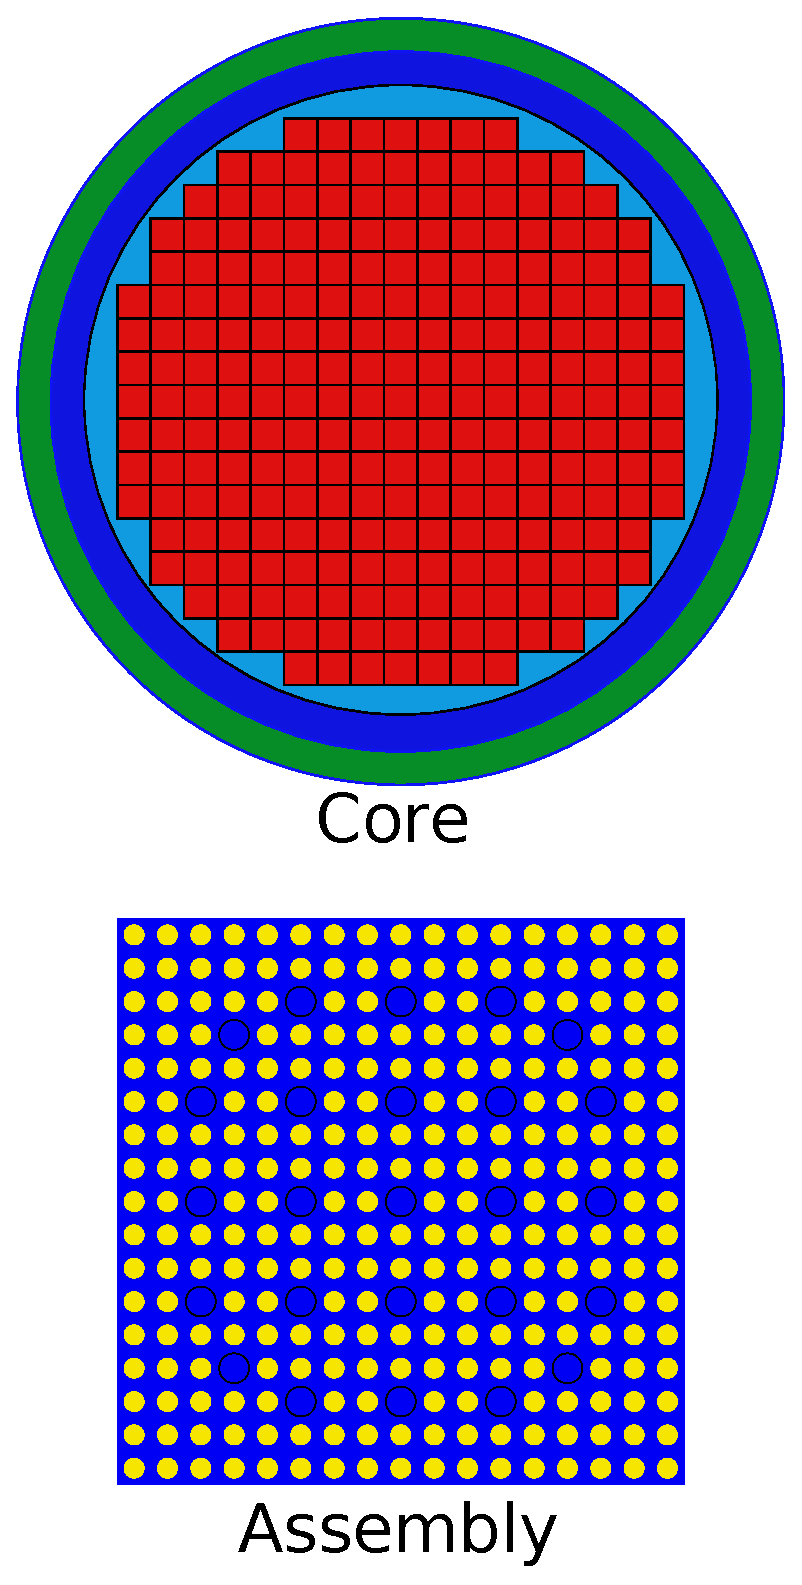
\includegraphics[width=2.5in]{mcperformance.eps}
  \caption{Geometry layout of the Monte Carlo Performance Benchmark.}
  \label{fig:core}
\end{figure}

A model of the Monte Carlo Performance Benchmark was built for both OpenMC and
MCNP5 based on Revision 1.2 of the benchmark specification. To get an estimate
of the effective multiplication factor, the MCNP model was run with 100,000
particles per cycle for 150 inactive and 1000 active batches. OpenMC was then
run with 100,000 particles per cycle, 150 inactive batches, and 4000 active
batches using the same ENDF/B-VII.0 libraries. \autoref{tab:mcperformance} shows
the effective multiplication factors and their standard deviations as reported
by the two codes. Once again, there is good agreement between OpenMC and MCNP
since the same cross section libraries were used.

\begin{table}
  \caption{Effective Multiplication Factor for the Monte Carlo Performance
    Benchmark Test.}
  \label{tab:mcperformance}
  \begin{center}
  \begin{tabular}{ l c }
    \hline
    Code & $k$-effective \\
    \hline
    MCNP5-1.51 & $1.00023 \pm 0.00006$ \\
    OpenMC     & $1.00002 \pm 0.00006$ \\
    \hline
  \end{tabular}
  \end{center}
\end{table}

\subsection{Tally performance}

The tally mapping technique described in Section \ref{sec:tallies} can help to
substantially reduce the overhead for scoring tallies when there are very large
numbers of scoring bins. To demonstrate this, we present some results concerning
tally overhead on the Monte Carlo Performance Benchmark model. This model has
been analyzed previously by \citet{mc21-physor} who showed a modest overhead for
large numbers of tallies when using techniques similar to those discussed here.

The Monte Carlo Performance Benchmark was run on an Intel Core i5 processor with
20,000 neutrons per cycle, 150 inactive batches, and 150 active batches. A mesh
tally was set up to score the neutron production rate over the entire core with
a single mesh cell covering every fuel pin divided into 100 axial segments. For
this model, such a mesh is 289 $\times$ 289 $\times$ 100 which in turn means
there are a total of 8,352,100 tally bins. The effective calculation rate was
4957 neutrons per second. \autoref{fig:tallies} shows the amount of time spent
in cycle during the simulation. One can see that each inactive cycle took on
average 3.79 s and each active cycle took on average 4.28 s, meaning
that the overhead due to tallies is about half a second per cycle. It is
interesting to note that almost all of the overhead is due to accumulating the
sum and sum-of-squares at the end of the cycle and not actually from the
subroutines in which individual particle histories score to the tally bins.

\begin{figure}[!ht]
  \centering
  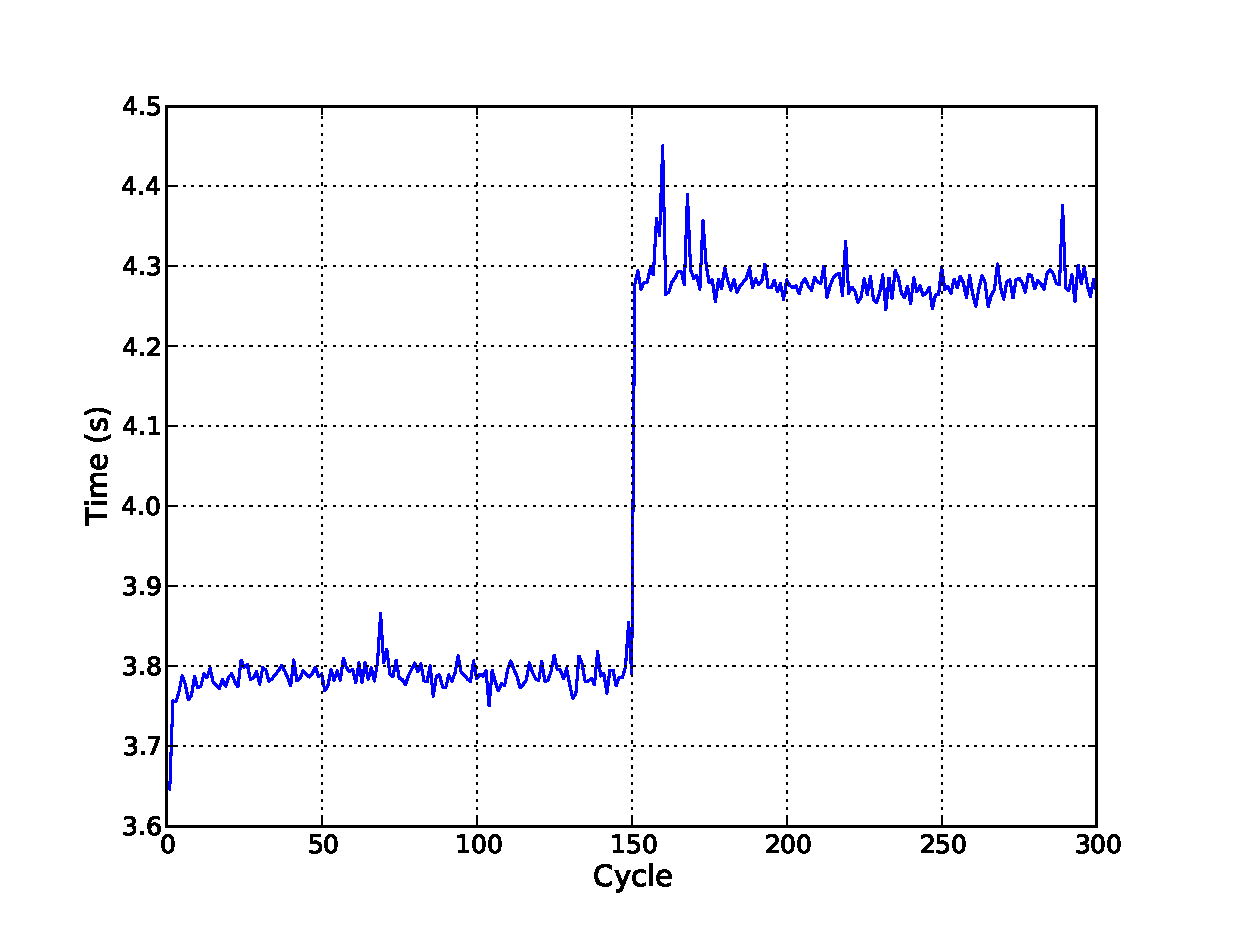
\includegraphics[width=4in]{tallies.eps}
  \caption{Elapsed cycle times with 8 million tally bins on Monte Carlo
    Performance Benchmark.}
  \label{fig:tallies}
\end{figure}

In general, the tally overhead will depend on many factors including the amount
of work per cycle, the total number of tally bins, the number of different
user-specified tallies, and how tallies are implemented in parallel runs. Thus,
the reader is cautioned from drawing any conclusions on a single study. The
example here was chosen merely to illustrate that OpenMC is indeed capable of
tallying millions of quantities with minimal overhead if properly
constructed. In this example, a single mesh had been used to cover all
fissionable regions. Had a separate mesh been used for each assembly in core,
the overhead may have been considerably higher. Similarly, had the run been
performed in parallel over hundreds of processors, there would be an additional
source of overhead from collecting the tallies onto one processor.

\subsection{Parallel scaling}

To test the parallel fission bank algorithm originally proposed by
\citet{fissionbank} and described further in Section \ref{sec:parallelism}, a
series of runs were performed on several different computer architectures to
test the scalability of OpenMC. Of most interest is the ability to scale on
large supercomputers with tens or hundreds of thousands of processors. Thus, the
Cray XK6 (Jaguar) supercomputer at Oak Ridge National Laboratory \citep{jaguar}
was chosen as the target system system for scaling studies.

The Monte Carlo Performance Benchmark was simulated using the Jaguar Cray XK6
system starting with 32 processors and increasing the processor count by a
factor of two up to 131,072 processors. For this study, the total work per
processor was kept constant (weak scaling) rather than the total amount of work
over all processors (strong scaling). For the 131,072 processor case, the total
number of particles per cycle was 2,621,440,000, equivalent to 20,000 particles
per processor per cycle.

\autoref{fig:scaling} shows the effective number of particles simulated per
second as a function of the number of processors in comparison to the ideal
calculation rate (assuming no communication between fission source
iterations). Excellent parallel efficiency is achieved even above 100,000
processors.

One should note that the effective number of particles per second reported in
\autoref{fig:scaling} does not take into account the initialization of the run
wherein the input files and cross sections must be read from disk or the
finalization of the run wherein tally statistics need to be computed and
subsequently written to disk. For a simulation on few processors, the
initialization and finalization time is generally insignificant compared to the
actual calculation time. However, with thousands of processors, the overhead
from initialization and finalization can become dominant if no changes are made
in the I/O algorithms. Future work at MIT will focus on implementing parallel
I/O techniques to mitigate this overhead.

\begin{figure}[!ht]
  \centering
  \includegraphics[width=4in]{scaling_loglog.eps}
  \caption{Parallel scaling for the Monte Carlo Performance Benchmark on the
    Cray XK6 (Jaguar) supercomputer.}
  \label{fig:scaling}
\end{figure}

\section{Conclusions}

A new Monte Carlo particle transport code called OpenMC has been developed to
study and help advance the state of particle simulations on high-performance
computing platforms. By choosing to adopt the ACE format for continuous-energy
neutron cross sections, the collision physics are faithful and contain very few
approximations. To appropriately model interactions in the thermal and
unresolved resonance energy ranges, one can use $S(\alpha,\beta)$ scattering law
data and unresolved resonance probability tables. All geometric objects are
represented using constructive solid geometry consisting of first- and
second-order surfaces. Together, the geometry and physics models make possible
high fidelity simulations of nuclear reactors.

Since OpenMC has been developed from scratch, the design and use of the code is
based on modern software design practices. This includes the use of an XML
format for user input that can be validated against a schema as well as HDF5
output that significantly simplifies post-processing and analysis of results
from the code. These design choices will help to lessen the learning-curve for
new developers and users.

Several benchmark results were presented comparing the effective multiplication
factor from OpenMC to that of MCNP5. These results show remarkable agreement and
demonstrate that the physics implementation can be considered validated for the
problem domains covered. In particular, the results on the pin-cell problem
\citep{pincell} and the Big Ten benchmark \citep{icsbep} demonstrate that the
implementation of $S(\alpha,\beta)$ thermal scattering models and the unresolved
resonance probability table method do not exhibit any obvious
deficiencies. Results on the Monte Carlo Performance Benchmark
\citep{hoogenboom} were presented to demonstrate the ability to model large
models with considerable geometric and material complexity.

The implementation of tallies in OpenMC was shown to be efficient with respect
to tallying large numbers of quantities thanks to a mapping technique that
allows for fast determination of scoring bin combinations. A test on the Monte
Carlo Performance Benchmark demonstrated that even with over 8 million tally
bins, the overhead was minimal. In addition to the excellent tally performance,
the parallel fission bank algorithm in OpenMC allows for parallel scaling up to
tens of thousands of processors.

The OpenMC Monte Carlo code has already become a central component of research
and development within MIT's Computational Reactor Physics Group and is being
used to actively support studies under the Center for Exascale Simulation and
Research. By releasing the code under an open source license, it is the authors'
hope that other members of the nuclear engineering community will become
involved and take advantage of the code for their own studies.

\section*{Acknowledgments}

This research was performed under appointment of the first author to the
Rickover Fellowship Program in Nuclear Engineering sponsored by Naval Reactor
Division of the US Department of Energy. Partial funding for this research was
provided by the Consortium for Advanced Simulation of Light Water Reactors, an
Energy Innovation Hub for Modeling and Simulation of Nuclear Reactors under US
Department of Energy Contract No. DE-AC05-00OR22725. The authors would also like
to thank Kord Smith and Andrew Siegel for the many fruitful discussions
regarding Monte Carlo simulation on exascale computing platforms.

\bibliography{references}
\bibliographystyle{annals}

\end{document}
